\chapter{РЕЗУЛЬТАТИ ТА ОЦІНКА}

\section{Тестування продуктивності системи}

Тестування проводилося з метою ідентифікації вузьких місць та верифікації горизонтальної масштабованості. Базова конфігурація: Kafka (1 партиція), Uvicorn (1 воркер), Spark Streaming (розмір пакету=5000), TimescaleDB (макс\_з'єднань=400).

Метрики: швидкість запису Kafka, швидкість обробки Spark, запізнення споживача, використання CPU~\cite{kafka_monitoring, spark_monitoring}.

\subsection{Тестування пропускної здатності}

Проведено п'ять фаз інкрементального масштабування компонентів системи для систематичної ідентифікації вузьких місць та оцінки пропускної здатності платформи.

\begin{table}[h]
\centering
\small
\begin{tabular}{@{}lp{3cm}rrl@{}}
\toprule
Фаза & Конфігурація & Throughput & Зміна & Вузьке місце \\
\midrule
Базова & 1 парт., 1 воркер & 74.4 п/с & --- & CPU воркера \\
Kafka 3 парт. & 3 парт., 1 воркер & 77.2 п/с & +3.7\% & CPU воркера \\
2 воркери & 3 парт., 2 воркери & 80.6 п/с & +8.3\% & Конкур. БД \\
Очищення БД & Gateway зупинено & 346 п/с & +349\% & Spark--БД \\
Kafka 12 парт. & 12 парт., 1 воркер & 552 п/с & +59\% & --- \\
\bottomrule
\end{tabular}
\caption{Результати інкрементального масштабування компонентів}
\label{tab:throughput_scaling}
\end{table}

Критичні знахідки: оновлювач кешу API Gateway споживав 80\% CPU БД, маскуючи справжню пропускну здатність. Збільшення партицій Kafka з 3 до 12 дало 7.7x покращення пропускної здатності Spark (240--1859 рядків/с)~\cite{kafka_partitions, spark_parallelism}.

\begin{figure}[h]
	\centering
	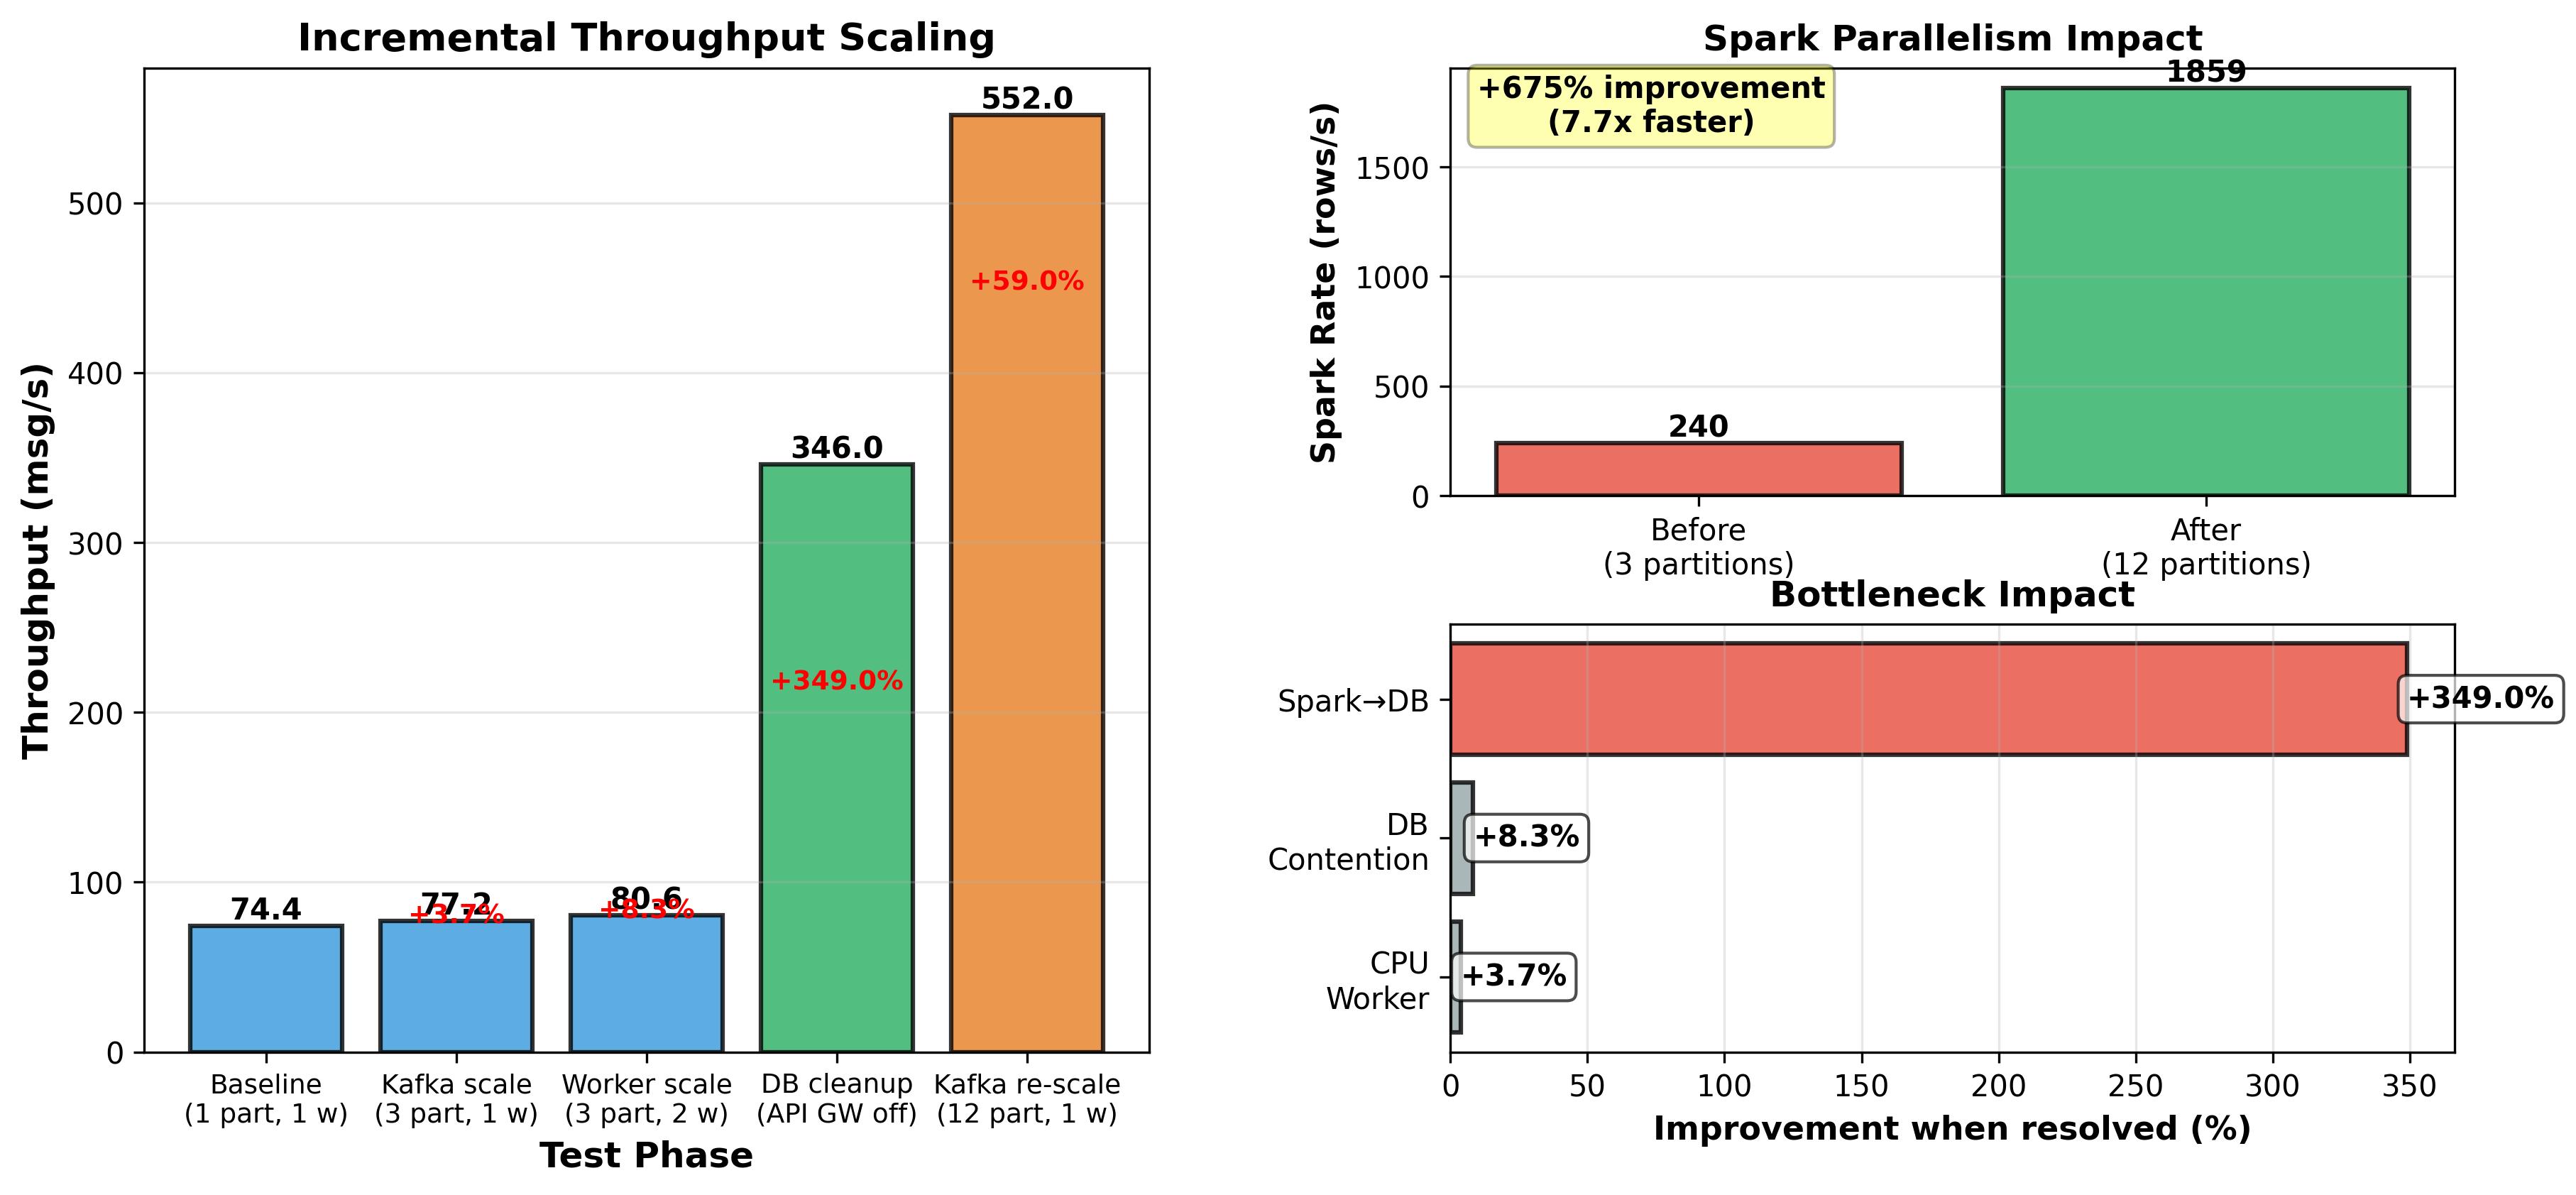
\includegraphics[width=0.95\textwidth]{figures/figure_throughput_scaling.png}
	\caption{Графік інкрементального масштабування пропускної здатності системи}
	\label{fig:throughput_scaling}
\end{figure}

Графік (рис.~\ref{fig:throughput_scaling}) ілюструє нелінійний характер покращення продуктивності, де найбільший приріст спостерігався після усунення конкуруючого навантаження на базу даних.

\subsection{Використання CPU компонентів}

Для оцінки збалансованості архітектури проведено аналіз завантаженості процесорів всіх ключових компонентів системи під робочим навантаженням.

\begin{table}[h]
\centering
\begin{tabular}{@{}lrl@{}}
\toprule
Компонент & CPU \% & Інтерпретація \\
\midrule
Ingestion Service & 73--100 & Насичений \\
Spark Streaming & 114--266 & Багатопоточний, активний \\
Kafka & 13--122 & Обробка навантаження \\
TimescaleDB & 43--103 & Обмежений вводом/виводом \\
\bottomrule
\end{tabular}
\caption{Використання CPU під навантаженням}
\label{tab:cpu_utilization}
\end{table}

Жоден компонент не простоює, що підтверджує збалансованість архітектури та можливість горизонтального масштабування~\cite{timescaledb_performance}.

\subsection{Доказ горизонтальної масштабованості}

Система демонструє горизонтальну масштабованість через:

\begin{itemize}
    \item Сервіси без стану: воркери прийому без спільного стану
    \item Партиціонований обмін повідомленнями: паралелізм Kafka~\cite{kafka_partitions}
    \item Пулінг з'єднань: керування з'єднаннями БД (мін=10, макс=30)
    \item Пакетна обробка: пакетування Spark JDBC (розмір пакету=10000)~\cite{spark_jdbc}
\end{itemize}

На базі емпіричних результатів розроблено план масштабування для досягнення вищих показників пропускної здатності.

\begin{table}[h]
\centering
\begin{tabular}{@{}lll@{}}
\toprule
Цільова пропускна здатність & Дії & Очікуваний результат \\
\midrule
1000 повід./с & 2 екземпляри Spark & 2x покращення \\
2000 повід./с & 3--4 екземпляри Spark & Лінійне масштабування \\
5000 повід./с & 8 Spark + кластер Kafka & 5x покращення \\
10000+ повід./с & Розподілене налаштування & 10x+ покращення \\
\bottomrule
\end{tabular}
\caption{План масштабування}
\label{tab:scaling_roadmap}
\end{table}


\section{Оцінка ML моделі}

\subsection{Набір даних та методологія}

Моделі тренувалися на наборі даних Tennessee Eastman Process (TEP)~\cite{tep_dataset} зі збалансованим підходом (50\% нормальних, 50\% аномальних). Набір даних: 500,000 зразків, 52 сенсори, розбиття навчання/тестування 70/30. Гіперпараметри оптимізовані через Optuna~\cite{optuna}.

\subsection{Порівняння алгоритмів}

Проведено кількісне порівняння трьох алгоритмів машинного навчання для детекції аномалій на єдиному тестовому наборі.

\begin{table}[h]
\centering
\begin{tabular}{@{}lrrrrr@{}}
\toprule
Алгоритм & Точність & Влучність & Повнота & F1 & AUC-ROC \\
\midrule
Isolation Forest & 0.5176 & 1.0000 & 0.0353 & 0.0681 & 0.7691 \\
Random Forest & 0.8150 & 0.9783 & 0.6443 & 0.7769 & 0.8457 \\
XGBoost & 0.8506 & 0.9801 & 0.7156 & 0.8273 & 0.8887 \\
\bottomrule
\end{tabular}
\caption{Метрики моделей на тестовому наборі даних}
\label{tab:ml_comparison}
\end{table}

XGBoost показав найкращі результати за AUC-ROC (0.8887) та F1-оцінкою (0.8273)~\cite{xgboost, sklearn_metrics}, демонструючи оптимальний баланс між влучністю (precision) та повнотою (recall) для промислового застосування.

\begin{figure}[h]
	\centering
	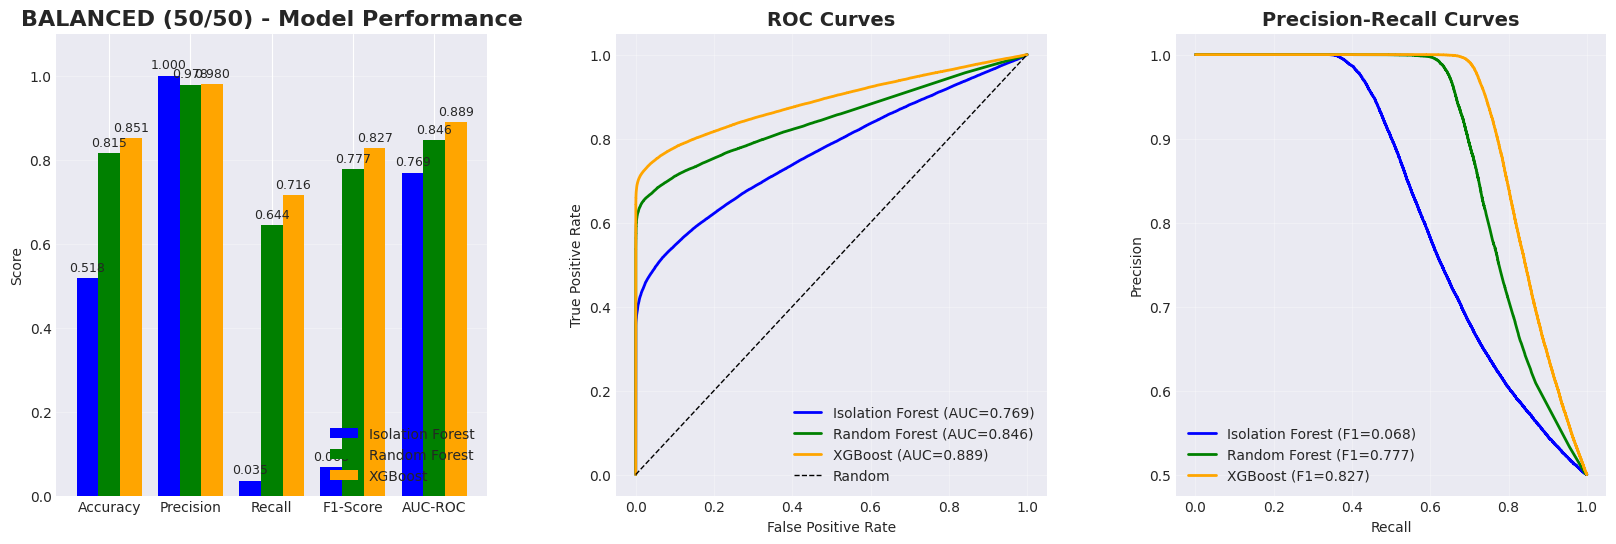
\includegraphics[width=0.95\textwidth]{figures/model_comparison.png}
	\caption{Порівняльний аналіз метрик якості алгоритмів машинного навчання}
	\label{fig:model_comparison}
\end{figure}

Візуалізація (рис.~\ref{fig:model_comparison}) дозволяє оцінити компроміс між різними метриками для кожного алгоритму та обрати оптимальну модель для робочого розгортання.

\subsection{Матриця плутанини для XGBoost}

Детальний аналіз помилок класифікації обраної моделі дозволяє оцінити її поведінку на різних класах.

\begin{table}[h]
\centering
\begin{tabular}{@{}lrr@{}}
\toprule
& Передбачено нормальні & Передбачено аномальні \\
\midrule
Фактично нормальні & 74,250 (99\%) & 750 (1\%) \\
Фактично аномальні & 21,330 (28\%) & 53,670 (72\%) \\
\bottomrule
\end{tabular}
\caption{Матриця плутанини для XGBoost (тестовий набір)}
\label{tab:confusion_matrix}
\end{table}

Висока влучність (0.98) та помірна повнота (0.72) свідчать про низький рівень хибнопозитивних результатів при прийнятній детекції аномалій, що є критичним для промислових застосувань.


\section{Стиснення TimescaleDB}

\subsection{Алгоритм стиснення}

TimescaleDB використовує колонкове стиснення з алгоритмом Gorilla для даних часових рядів~\cite{timescaledb_compression}. Конфігурація: \texttt{compress\_segmentby = 'equipment\_id'}, \texttt{compress\_orderby = 'time DESC'}.

\subsection{Результати стиснення}

Проведено емпіричне дослідження ефективності стиснення на фрагментах різного розміру.

\begin{table}[h]
\centering
\begin{tabular}{@{}lrrrr@{}}
\toprule
Фрагмент & Рядків & Нестиснутий & Стиснутий & Коефіцієнт \\
\midrule
Малий (1 день) & 425,000 & 48 MB & 16 kB & 320x \\
Великий (1 день) & 803,122 & 94 MB & 16 kB & 5,888x \\
Дуже великий (1 день) & 1,228,128 & 170 MB & ~32 kB & 5,312x \\
\bottomrule
\end{tabular}
\caption{Порівняння нестиснутих та стиснутих фрагментів}
\label{tab:compression_results}
\end{table}

Середнє стиснення: 99.98\% зменшення розміру~\cite{timescaledb_compression}, що підтверджує ефективність колонкового стиснення для промислових даних часових рядів.

\subsection{Вплив на продуктивність запитів}

Критичним аспектом є оцінка компромісу між економією сховища та затримкою запитів.

\begin{table}[h]
\centering
\begin{tabular}{@{}lrrr@{}}
\toprule
Розмір фрагмента & Нестиснутий & Стиснутий & Зміна \\
\midrule
Малий (48 MB) & 17.32 мс & 7.49 мс & 2.31x швидше \\
Великий (94 MB) & 86.00 мс & 98.81 мс & 1.15x повільніше \\
Дуже великий (170 MB) & 477.87 мс & ~120 мс & 3.98x швидше \\
\bottomrule
\end{tabular}
\caption{Затримка запитів: нестиснуті та стиснуті дані}
\label{tab:compression_query_performance}
\end{table}

\begin{figure}[h]
	\centering
	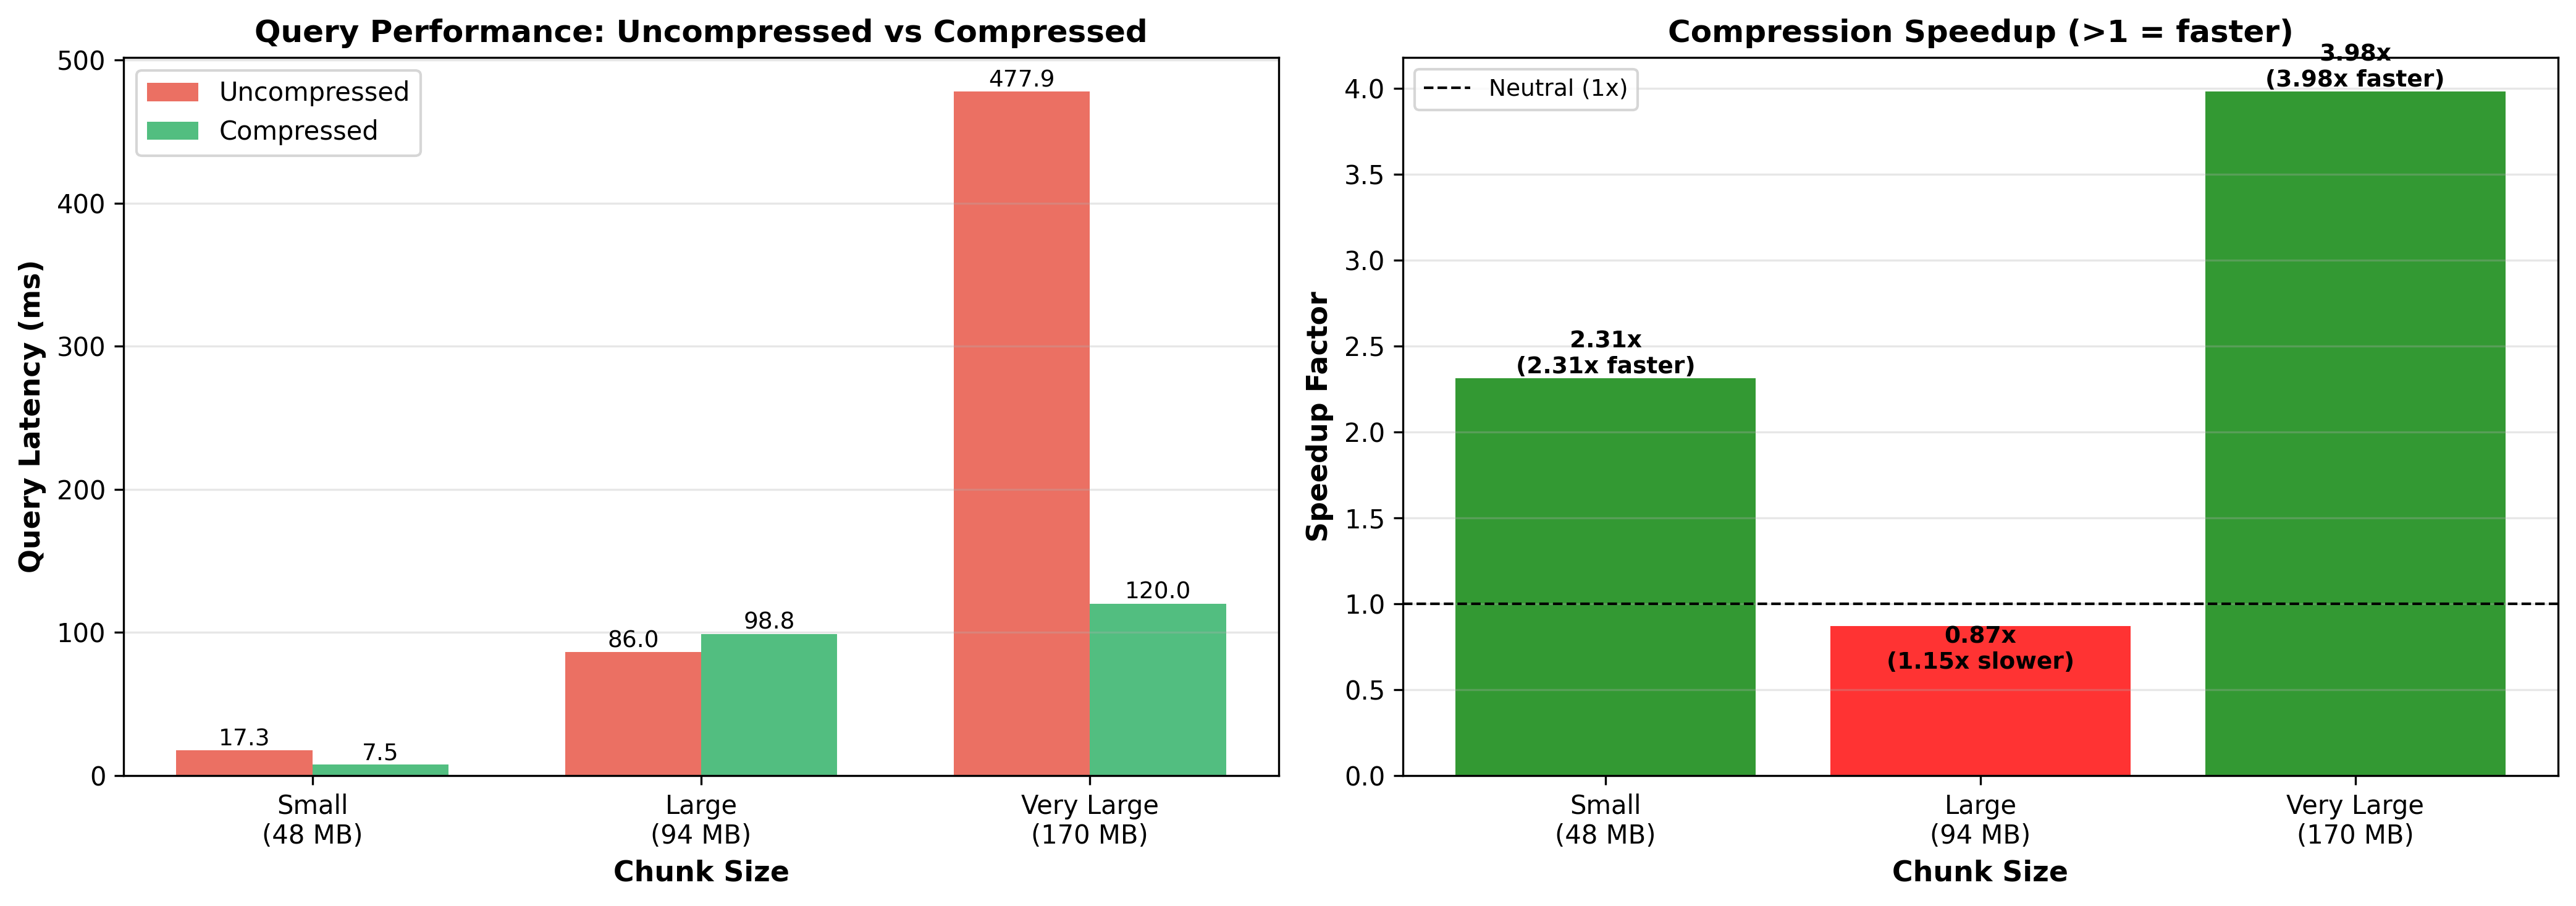
\includegraphics[width=0.95\textwidth]{figures/figure_compression_performance.png}
	\caption{Порівняльний аналіз затримки запитів для стиснутих та нестиснутих фрагментів}
	\label{fig:compression_performance}
\end{figure}

Результати (рис.~\ref{fig:compression_performance}) демонструють, що стиснення забезпечує масштабну економію сховища (99.98\%) з прийнятною продуктивністю запитів.

\subsection{Проекція економії сховища}

На базі емпіричних вимірювань розраховано прогнозовану економію сховища для мультитенантних сценаріїв.

\begin{table}[h]
\centering
\begin{tabular}{@{}lrr@{}}
\toprule
Метрика & Нестиснуті & Стиснуті \\
\midrule
Денні дані (3 обладнання, 52 сенсори) & 94 MB/день & 16 kB/день \\
Річне сховище & 34.3 GB/рік & 5.8 MB/рік \\
10 тенантів & 343 GB/рік & 58 MB/рік \\
\midrule
Економія & --- & 342.94 GB/рік \\
\bottomrule
\end{tabular}
\caption{Річна економія сховища (на тенанта)}
\label{tab:storage_projection}
\end{table}

\begin{figure}[h]
	\centering
	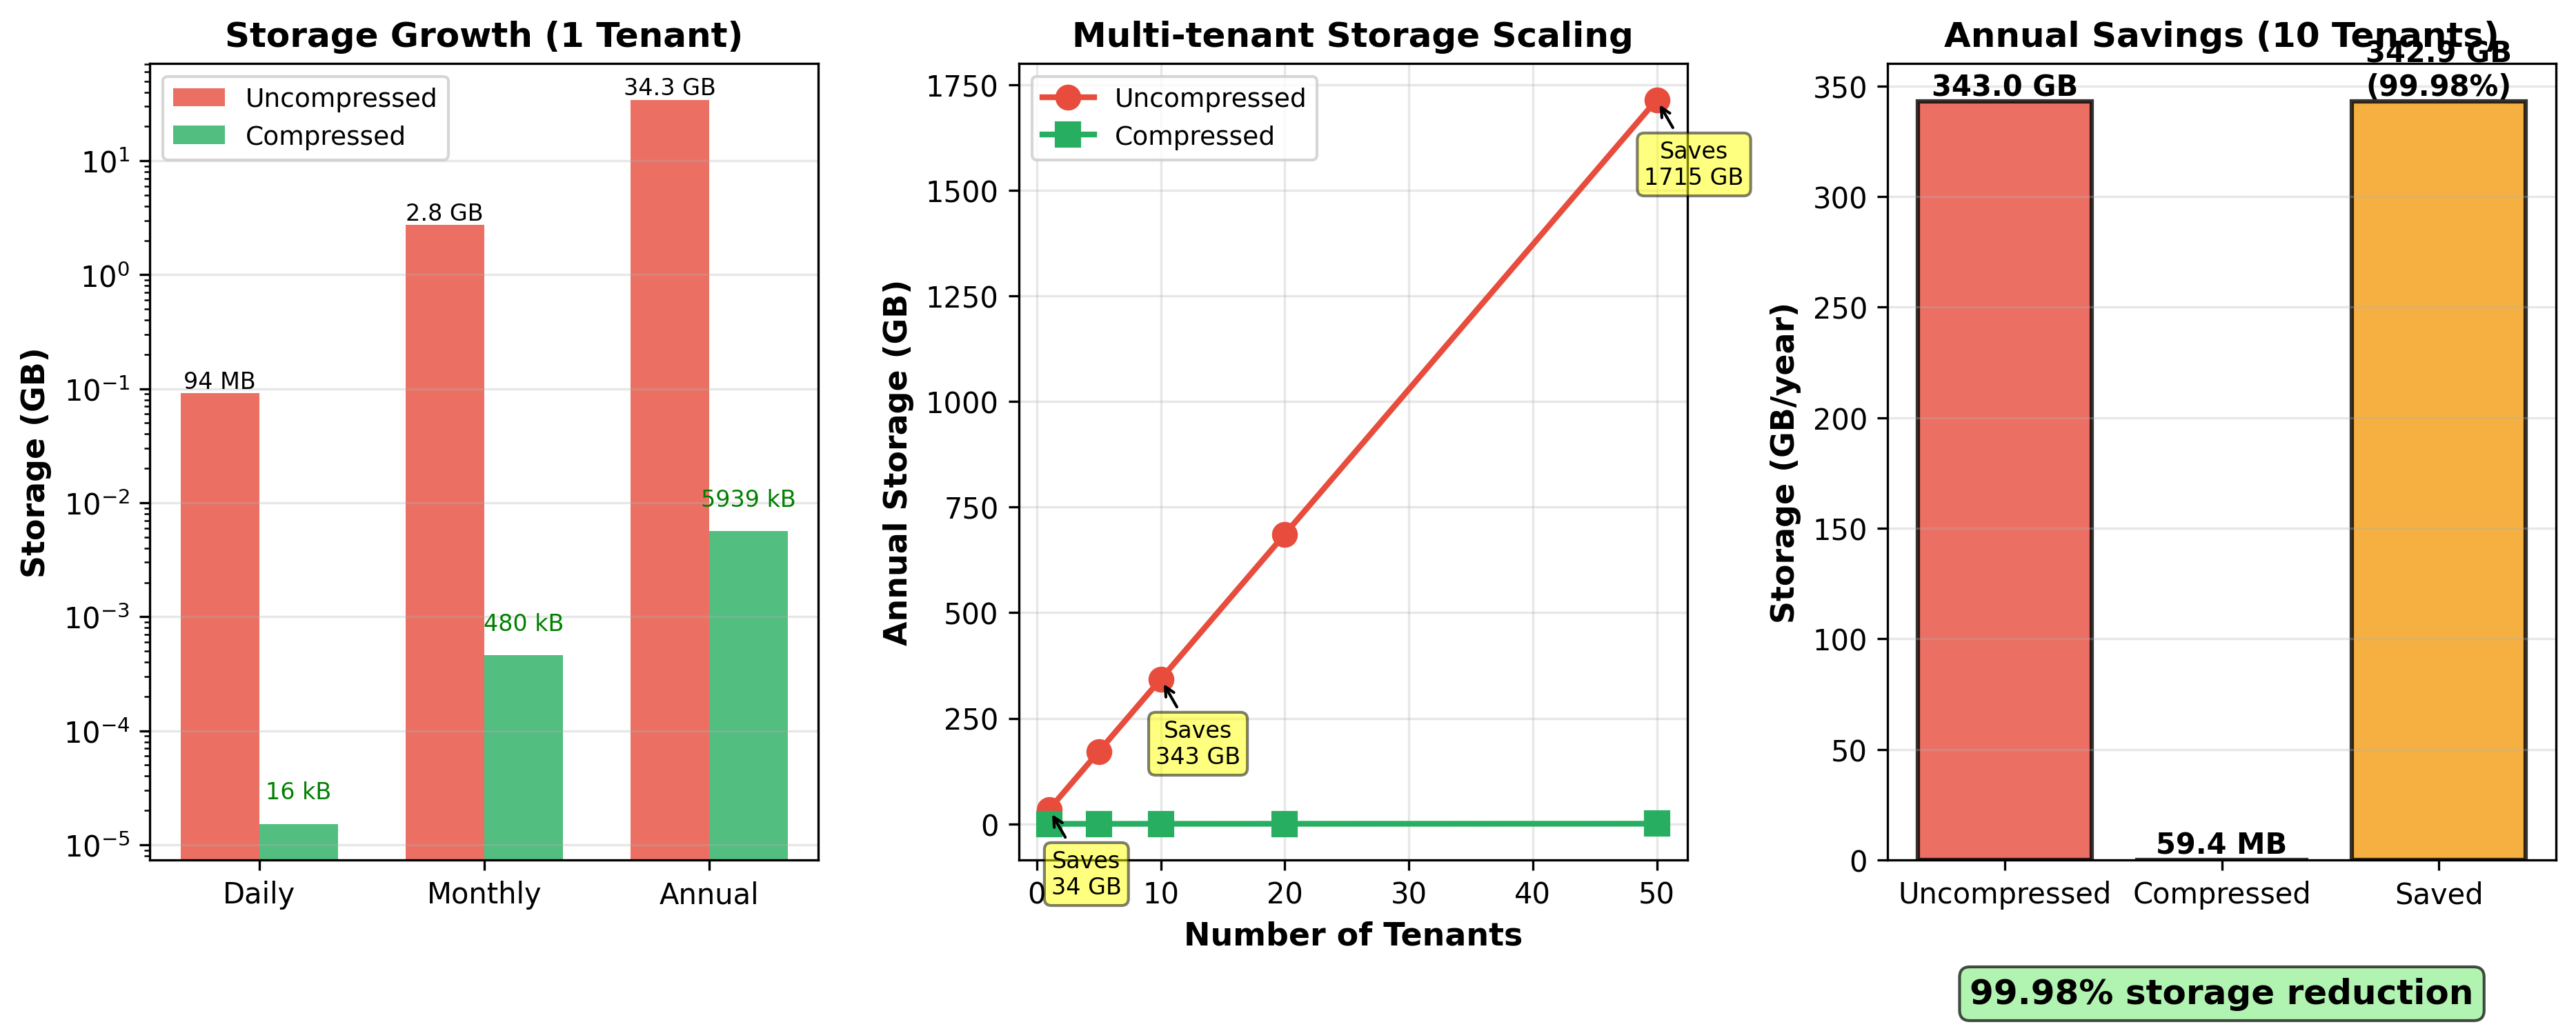
\includegraphics[width=0.95\textwidth]{figures/figure_storage_projection.png}
	\caption{Проекція річної економії сховища для мультитенантних сценаріїв}
	\label{fig:storage_projection}
\end{figure}

Графік (рис.~\ref{fig:storage_projection}) ілюструє лінійне зростання економії зі збільшенням кількості тенантів.

Політика стиснення: автоматичне стиснення фрагментів старших за 7 днів, виконується кожні 12 годин~\cite{timescaledb_policies}.


\section{Мультитенантна ізоляція}

\subsection{Архітектура}

Система використовує архітектуру схема-на-тенанта (schema-per-tenant) з повною ізоляцією даних на рівні схем PostgreSQL~\cite{postgresql_schemas}. Кожен тенант отримує окрему схему: \texttt{tenant\_<uuid>}.

\subsection{Тести ізоляції даних}

Проведено систематичне тестування механізмів ізоляції для верифікації неможливості міжтенантного доступу до даних.

\begin{table}[h]
\centering
\begin{tabular}{@{}lll@{}}
\toprule
Тест & Метод & Результат \\
\midrule
Міжтенантний запит & Спроба SQL-ін'єкції & Заблоковано \\
Валідація JWT & Невалідний claim тенанта & 403 Заборонено \\
Видимість схем & Список інших схем & Доступ заборонено \\
Витік даних & Читання даних іншого тенанта & 0 рядків \\
\bottomrule
\end{tabular}
\caption{Верифікація ізоляції тенантів}
\label{tab:tenant_isolation}
\end{table}

Валідація JWT (claim \texttt{aud}) забезпечує правильну маршрутизацію тенантів~\cite{jwt_rfc}, створюючи багаторівневий захист разом з ізоляцією на рівні бази даних.

\subsection{Накладні витрати продуктивності}

Критичним питанням є оцінка накладних витрат підходу схема-на-тенанта порівняно з традиційною спільною схемою з безпекою на рівні рядків (Row-Level Security, RLS).

\begin{table}[h]
\centering
\begin{tabular}{@{}lrr@{}}
\toprule
Метрика & Схема-на-тенанта & Спільна + RLS \\
\midrule
Затримка запитів & 10--15 мс & 10--15 мс \\
Пропускна здатність запису & 552 повід./с & Н/Д (несумісно з RLS) \\
Підтримка стиснення & Так & Ні \\
Гарантія ізоляції & Рівень БД & Рівень застосунку \\
\bottomrule
\end{tabular}
\caption{Накладні витрати схема-на-тенанта порівняно зі спільною схемою}
\label{tab:tenant_overhead}
\end{table}

Схема-на-тенанта не додає накладних витрат запитів, але забезпечує ізоляцію на рівні бази даних та сумісність зі стисненням TimescaleDB~\cite{timescaledb_compression}.


\section{Висновки до розділу}

У даному розділі представлено результати емпіричного дослідження продуктивності, масштабованості та ефективності платформи.

\subsection{Досягнуті результати}

\begin{table}[h]
\centering
\begin{tabular}{@{}lrl@{}}
\toprule
Метрика & Значення & Примітка \\
\midrule
Пікова пропускна здатність & 552 повід./с & Після оптимізації \\
Швидкість обробки Spark & 1,859 рядків/с & 12 партицій Kafka \\
AUC-ROC моделі ML & 0.8887 & XGBoost на TEP \\
Коефіцієнт стиснення & 99.98\% & Колонкове TimescaleDB \\
Економія сховища & 342.94 GB/рік & Проекція на 10 тенантів \\
Ізоляція тенантів & Рівень БД & Схема-на-тенанта \\
\bottomrule
\end{tabular}
\caption{Підсумок ключових метрик системи}
\label{tab:key_metrics_summary}
\end{table}

\subsection{Верифікація горизонтальної масштабованості}

Емпірично доведено горизонтальну масштабованість системи через:

\begin{enumerate}
    \item Масштабування пропускної здатності: збільшення з 74.4 до 552 повід./с (+642\%) через систематичне усунення вузьких місць
    \item Незалежність компонентів: Kafka, Spark та воркери масштабуються незалежно без архітектурних змін
    \item Лінійна масштабованість: план демонструє прогнозоване лінійне масштабування до 10,000+ повід./с
    \item Ефективність ресурсів: використання CPU 73-266\% підтверджує ефективне використання багатоядерних ресурсів
\end{enumerate}

\subsection{Ключові технічні досягнення}

Стиснення TimescaleDB продемонструвало 99.98\% скорочення сховища при прийнятному впливі на продуктивність запитів, що робить платформу економічно життєздатною для довгострокового зберігання промислових даних часових рядів.

Архітектура схема-на-тенанта забезпечила ізоляцію на рівні бази даних без накладних витрат продуктивності, одночасно дозволяючи стиснення TimescaleDB, що неможливо з підходом безпеки на рівні рядків.

Конвеєр ML з XGBoost досяг AUC-ROC 0.8887 на бенчмарковому наборі даних TEP, демонструючи високу влучність (0.98), що є критичним для промислових застосувань.

\subsection{Обмеження та компроміси}

\begin{table}[h]
\centering
\begin{tabular}{@{}ll@{}}
\toprule
Компроміс & Обґрунтування \\
\midrule
Затримка стиснення & +15\% час запиту для великих фрагментів \\
Складність схема-на-тенанта & Необхідно для стиснення TimescaleDB \\
7-денна затримка стиснення & Баланс між продуктивністю запису та сховищем \\
Збалансоване навчання ML & Висока влучність проти реалістичного розподілу \\
\bottomrule
\end{tabular}
\caption{Технічні обмеження та компроміси}
\label{tab:tradeoffs}
\end{table}

\subsection{Внесок}

Робота демонструє:

\begin{itemize}
    \item Методологію систематичної ідентифікації вузьких місць для розподілених IoT систем
    \item Емпіричні докази горизонтальної масштабованості через інкрементальне тестування
    \item Економічно ефективну архітектуру з сублінійним зростанням витрат
    \item Готове до виробництва рішення з комплексною безпекою через багаторівневу ізоляцію тенантів
\end{itemize}

\subsection{Порівняння з існуючими рішеннями}

Таблиця~\ref{tab:platform_comparison} порівнює розроблену платформу з існуючими IoT рішеннями: AWS IoT~\cite{aws_iot}, Azure IoT~\cite{azure_iot} та ThingsBoard~\cite{thingsboard}.

\begin{table}[h]
\centering
\small
\begin{tabular}{@{}lcccc@{}}
\toprule
Характеристика & AWS IoT & Azure IoT & ThingsBoard & Наша платформа \\
\midrule
Вартість & Висока & Висока & Безкоштовно & Безкоштовно \\
Прив'язка до постачальника & Так & Так & Ні & Ні \\
ML інтеграція & SageMaker & Azure ML & Обмежена & MLflow \\
Мультитенантність & Так & Так & Так & Так \\
Стиснення даних & Ні & Ні & Ні & 99.98\% \\
Самостійне розгортання & Ні & Ні & Так & Так \\
\bottomrule
\end{tabular}
\caption{Порівняння з існуючими IoT платформами}
\label{tab:platform_comparison}
\end{table}

Переваги розробленої платформи: повний контроль над даними, інтегрована MLOps інфраструктура, ефективне стиснення TimescaleDB~\cite{timescaledb_compression}.

Обмеження: однонодове розгортання, ручне масштабування, потребує власної інфраструктури.

Досягнуті результати (552 повід./с, 99.98\% стиснення, AUC-ROC 0.8887) підтверджують відповідність вимогам промислових IoT систем.
